\section{The Calorimeters}
\label{sec:calo}

\subsection{Electromagnetic Calorimeter}

Particles that survive the Tracker will then encounter the Electromagnetic Calorimeter (ECAL).
The ECAL is a hermetic homogeneous sub-detector consisting of a barrel part (EB) and two endcap parts (EE).
The EB contains 61200 lead tungstate (PbWO$_4$) crystals while each EE contains 7324 crystals.
Due to its short radiation length (0.89 cm) and high density (8.28 g/cm$^3$),
PbWO$_4$ is a good material to use in the ECAL.
Conveniently after 1 bunch crossing (25 ns), nearly 80\% of the scintillated light is emitted.

\begin{figure*}[!htb]
    \centering
    \captionsetup{justification=justified}
    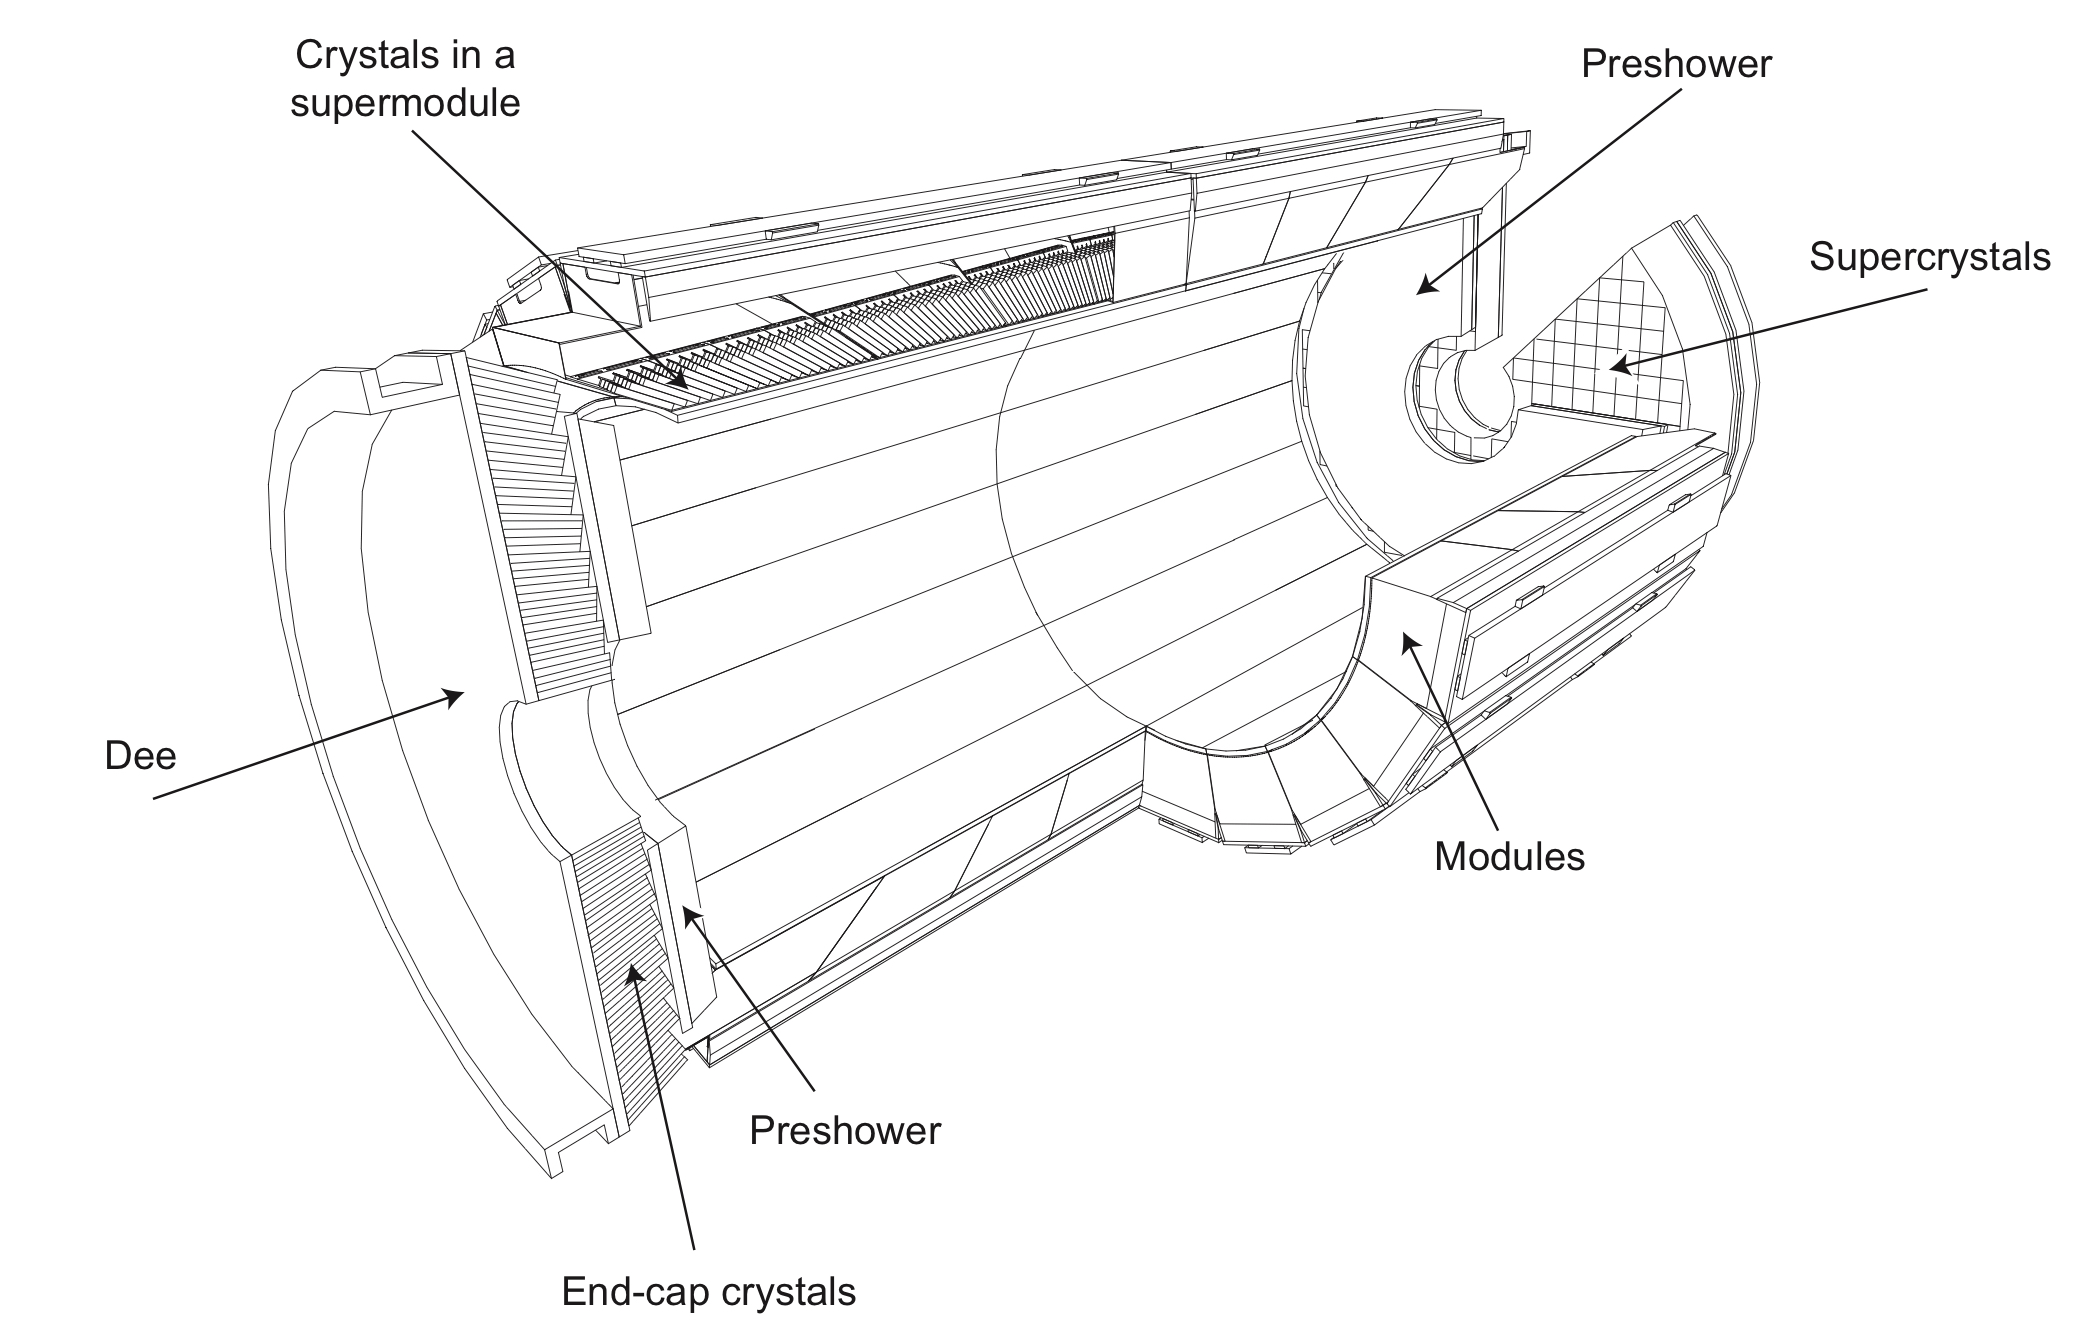
\includegraphics[width=0.95\textwidth]{figures/ECAL/xs_whiteblack.jpeg}
    \caption{Cross sectional view of the electromagnetic calorimeter of CMS.
             Figure taken from Ref.~\cite{jinst:cms_exp}.}
    \label{fig:ecal_xs}
\end{figure*}

whose purpose is to absorb photons and electrons and detect their energies and directions.

\subsection{Hadronic Calorimeter}

